\documentclass[compress]{beamer}
%
% Choose how your presentation looks.
%
% For more themes, color themes and font themes, see:
% http://deic.uab.es/~iblanes/beamer_gallery/index_by_theme.html
%
\mode<presentation>
{
	\usetheme{Dresden}      % or try Darmstadt, Madrid, Warsaw, ...  
	%\useoutertheme{infolines} % split, tree, infolines
	%\useinnertheme{rectangles}
	\usecolortheme{orchid} % or try albatross, beaver, crane, ...
	\usefonttheme{structuresmallcapsserif}  % or try serif, structurebold, ...
	\setbeamertemplate{navigation symbols}{}
	\setbeamertemplate{caption}[numbered]
	\setbeamertemplate{footline}[frame number]
} 

\usepackage[english]{babel}
\usepackage[utf8]{inputenc}
\usepackage{tikz}
\usetikzlibrary{trees,snakes,arrows}
\usepackage{tabularx}
\usepackage{subfig}
\usepackage{graphicx}
\usepackage{arydshln} %for dashed lines
\usepackage{booktabs} %for top-/bottom-/midrule
\usepackage{standalone}
\usepackage{hyperref}



%\usepackage[backend=bibtex, citestyle=numeric, bibstyle=authoryear, sorting=none, autocite=superscript, labeldateparts]{biblatex}
%\addbibresource{bibliography.bib}
%
%% Script to get consistent cite numbering
%%%%%%%%%%%%%%%%%%%%%%%%%%%%%%%%%%%%%%%%%%%%%%%%%%%%%%%%%%%%%%
%\newbibmacro*{aycite:shorthand}{%
%	\printtext[bibhyperref]{\printfield{shorthand}}}
%
%\newbibmacro*{aycite:label}{%
%	\iffieldundef{label}
%	{\printtext[bibhyperref]{\printfield[citetitle]{labeltitle}}}
%	{\printtext[bibhyperref]{\printfield{label}}}}
%
%\newbibmacro*{aycite:labelyear+extrayear}{%
%	\iffieldundef{labelyear}
%	{}
%	{\printtext[bibhyperref]{\printlabeldateextra}}}
%
%\newbibmacro*{aycite}{%
%	\iffieldundef{shorthand}
%	{\ifthenelse{\ifnameundef{labelname}\OR\iffieldundef{labelyear}}
%		{\usebibmacro{aycite:label}%
%			\setunit{\printdelim{nonameyeardelim}}}
%		{\printnames{labelname}%
%			\setunit{\printdelim{nameyeardelim}}}%
%		\usebibmacro{aycite:labelyear+extrayear}}
%	{\usebibmacro{aycite:shorthand}}}
%
%\DeclareCiteCommand{\supercite}
%{}
%{\footnote[\thefield{labelnumber}]{\usebibmacro{prenote}\usebibmacro{aycite}\usebibmacro{postnote}}}
%{\supercitedelim}
%{}
%
%% Smaller citations
%\renewcommand{\footnotesize}{\tiny}
%%%%%%%%%%%%%%%%%%%%%%%%%%%%%%%%%%%%%%%%%%%%%%%%%%%%


\def\tobar{\mathrel{\mkern3mu  \vcenter{\hbox{$\scriptscriptstyle+$}}%
		\mkern-12mu{\to}}}

\usepackage{alphalph}
\renewcommand*{\thesubfigure}{%
	\alphalph{\value{subfigure}}%
}%

\title[BA Hobbhahn 2019]{Object Detection using the Scattering Transform}
\author{Marius Hobbhahn}
\date{\today}

\begin{document}
	
	\begin{frame}
		\titlepage
	\end{frame}
	%
	% Uncomment these lines for an automatically generated outline.
	%\begin{frame}{Outline}
	%  \tableofcontents
	%\end{frame}
	%
	\section{Introduction}
	\subsection{ } % for the dots - there most probably is a more elegant solution.
	%
	\begin{frame}{Motivation}
		\begin{block}{Problems}
			\begin{enumerate}
				\item Loads of data necessary for training
				\item Capability to generalize unclear for different circumstances (i.e. equivariances and invariances w.r.t. some transformations)
			\end{enumerate}
		\end{block}
		\begin{block}{Possible solutions}
			\begin{enumerate}
				\item Filters that generalize quickly
				\item Filters that are globally equivariant and locally invariant w.r.t. some transformations, i.e. translation, rotation, scale 
			\end{enumerate}
		\end{block}
	\end{frame}
	%
	\begin{frame}{Scattering Transform}
		\begin{block}{Basic Idea}
			Static image filter that has certain theoretical guarantees with respect to global equivariances and local invariances (i.e. translation, scale, rotation).
		\end{block}
		\begin{equation}
		\psi(u) = C_1 (e^{iu.\xi} - C_2) e^{\frac{-|u|^2}{2\sigma^2}}
		\label{eq:morlet2d}
		\end{equation}
		\begin{itemize}
			\item $\xi$: central frequency ($3\pi/4$)
			\item $\sigma$: width of the Gaussian part ($0.85$)
			\item $C_1, C_2$: Constants, $C_2$ is chosen s.t. $\int \psi(u)du = 0$ and $C_1 = 1$
		\end{itemize}
	\end{frame}
	%
	%what is U
	%what is f
	%what is \phi
	%what is S
	%what is \lambda
	%
	\begin{frame}{Visualization of the Scattering Transform}
		\begin{figure}
			\centering
			\begin{tabular}{cc}
				\subfloat[]{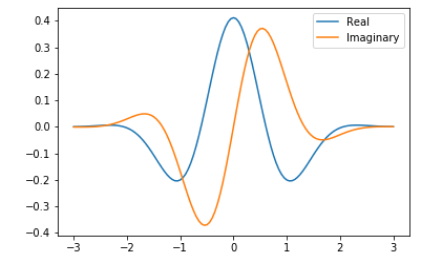
\includegraphics[width=6cm]{images/Morlet_wavelet_1D.png}} 
				& \subfloat[]{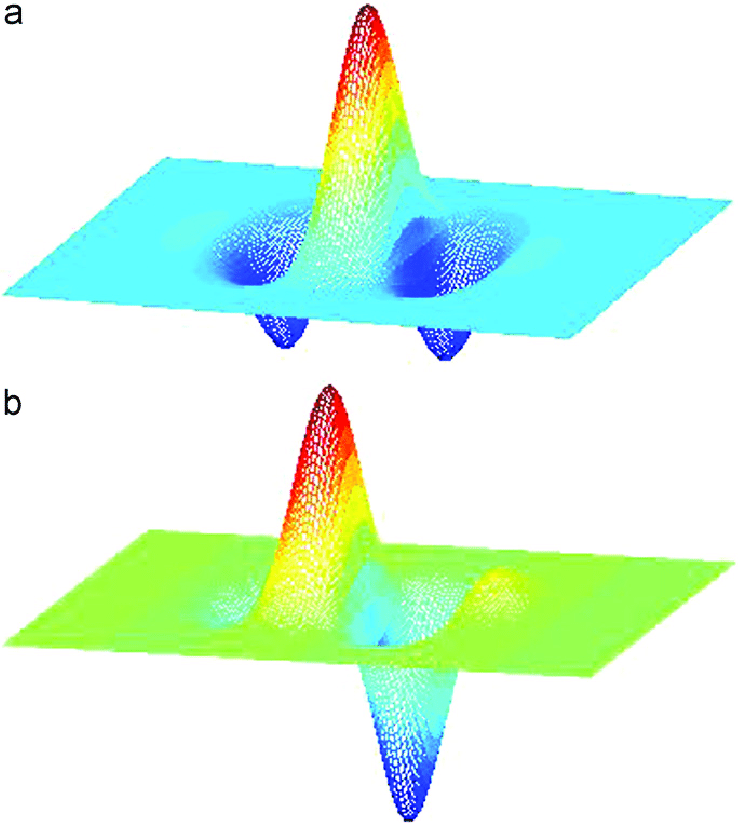
\includegraphics[width=4cm]{images/2D-Morlet-wavelet-a-Real-part-b-Imaginary-part.png}}
			\end{tabular}
			\caption{Complex Morlet wavelet in 1D and 2D}
		\end{figure}
	\end{frame}
	
	\begin{frame}{Visualization of the filter bank}
		\begin{minipage}[c]{0.67\textwidth}
			\begin{figure}[!htb]
				\centering
				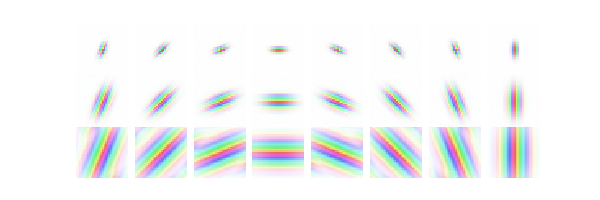
\includegraphics[width=1\textwidth]{images/filter_bank_vis.png}
				\caption{Visualization of the filter bank. $j=3$ is denotes the down scale factor and $\theta=8$ the number of angles. Color saturation and color hue respectively denote complex magnitude and complex phase.}
				\label{fig:viz_filter_bank}
			\end{figure}
		\end{minipage}\hfill
		\begin{minipage}[r]{0.32\textwidth}
			\begin{figure}[!htb]
				\centering
				
\includegraphics[width=1.2\textwidth]{images/low_pass_vis.png}
				\caption{Visualization of the low pass (Gaussian) Filter}
				\label{fig:viz_low_pass}
			\end{figure}
		\end{minipage}
	\end{frame}
	%
	\begin{frame}{Scattering Networks}
		\begin{block}{Basic Idea}
			Apply the scattering transform multiple times to get higher order scattering coefficients.
		\end{block}
		\begin{figure}[!htb]
			\centering
			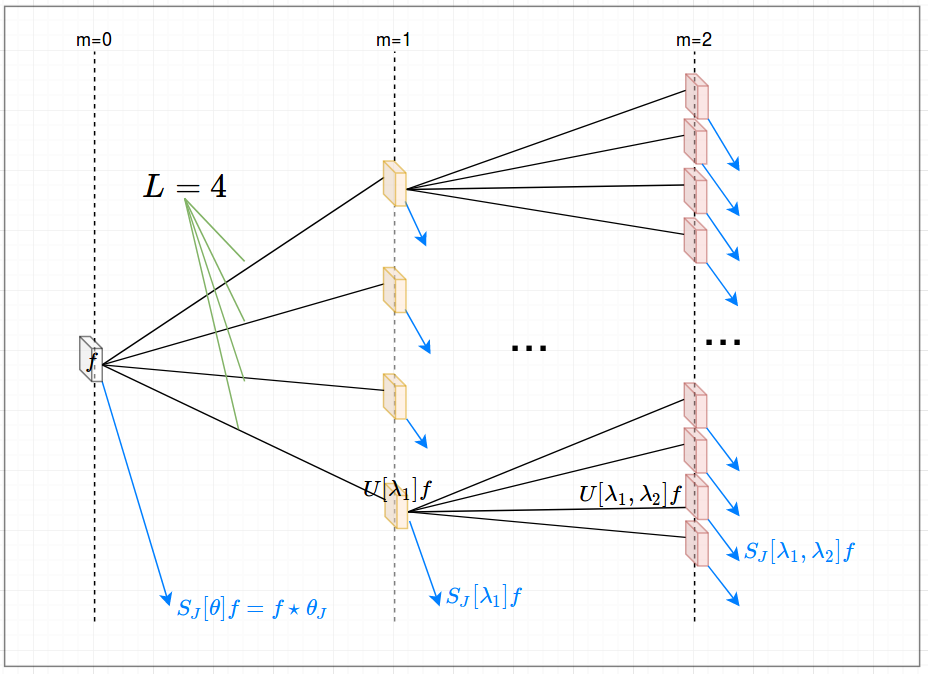
\includegraphics[width = 0.7\textwidth]{images/scattering_network_overview.png}
			\caption{}
			\label{fig:scattering_network}
		\end{figure}
	\end{frame}
	%
	\begin{frame}{Example}
		\begin{minipage}[c]{0.67\textwidth}
		\begin{figure}[!htb]
			\begin{tabular}{cc}
				\subfloat[]{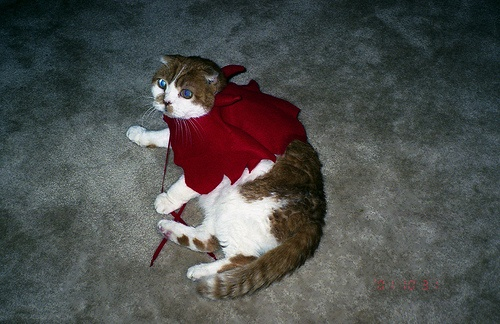
\includegraphics[width=2.5cm]{images/cat_example.jpg}} 
				& \subfloat[]{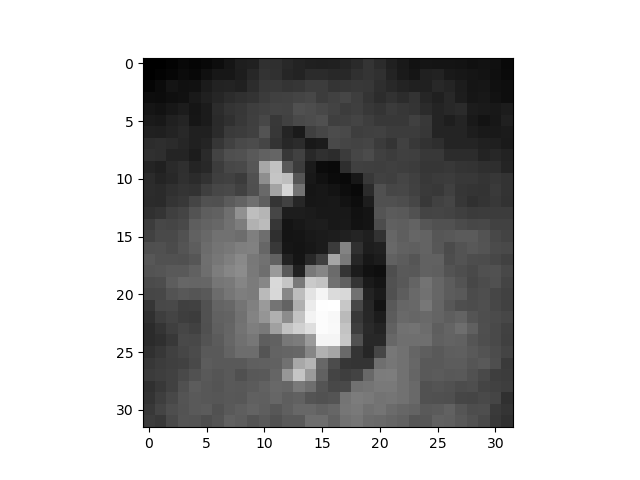
\includegraphics[width=3cm]{images/example_cat_0ord.png}}\\
				
				\subfloat[]{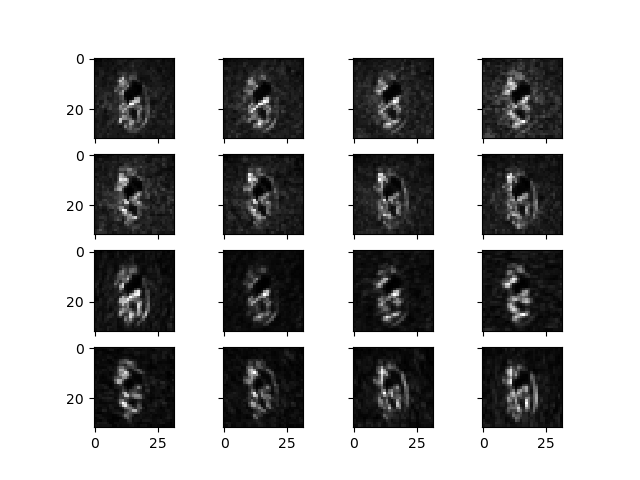
\includegraphics[width=4cm]{images/example_cat_1ord.png}} &
				\subfloat[]{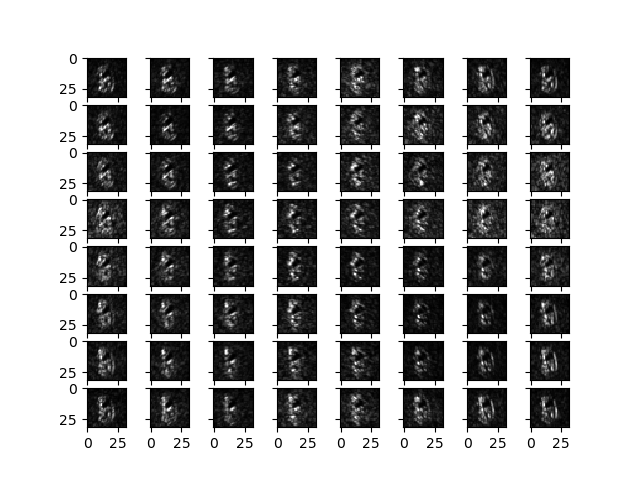
\includegraphics[width=4cm]{images/example_cat_2ord.png}}
			\end{tabular}
			%\caption{Image taken from the VOC dataset. a) Original image; b) 0th order scattering coefficients, i.e. a Gaussian low-pass filter; c) First order scattering coefficients; d) Second order scattering coefficients}
			\label{fig:example_cat_coefficients}
		\end{figure}
		\end{minipage}\hfill
		\begin{minipage}[c]{0.3\textwidth}
		\begin{itemize}
			\item Example for $L=8, J=2, N, M = 128$
			\item a) original image
			\item b) Gaussian low-pass filter
			\item c) first order scattering coefficients (size 32x32)
			\item d) second order scattering coefficients (size 32x32)
		\end{itemize}			
		\end{minipage}
	\end{frame}
	%
	\begin{frame}{Properties of the Scattering Transform}
		\begin{minipage}[c]{0.67\textwidth}
		\begin{figure}
			\centering
			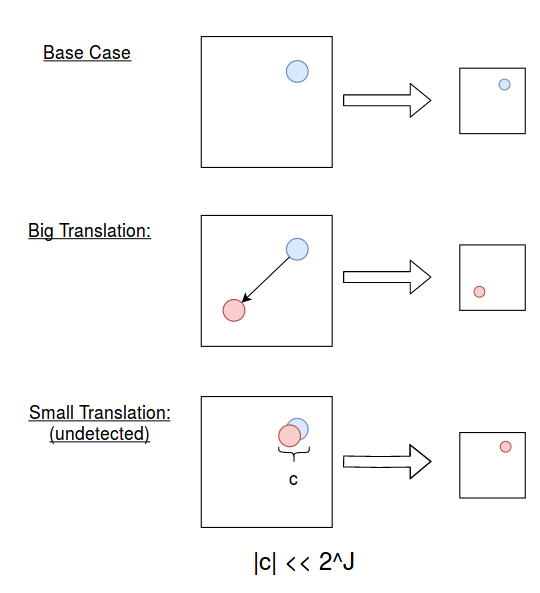
\includegraphics[width=\textwidth]{images/equiv_inv.png}
		\end{figure}
		\end{minipage}\hfill
		\begin{minipage}[c]{0.3\textwidth}
			\begin{itemize}
				\item Invariance: $f(Tx) = f(x)$
				\item Equivariance: $f(Tx) = Tf(x)$
				\item Local invariance but global equivariance 
			\end{itemize}			
		\end{minipage}
	\end{frame}
	%
	\begin{frame}{Hybrid scattering networks for classification}
		\begin{figure}
			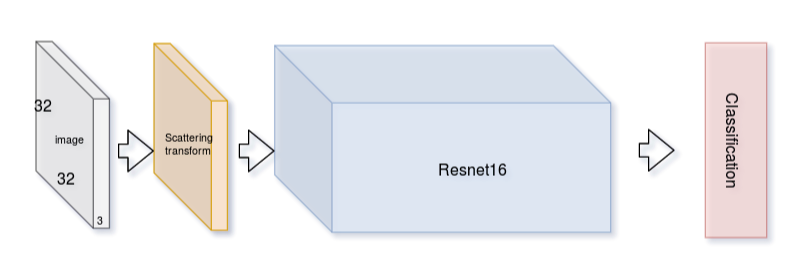
\includegraphics[width=0.9\textwidth]{images/arch_hybrid_scattering_CIFAR10.png}
			\caption{Architecture \cite{ScalingTheScatteringTransform2017}}
		\end{figure}
		\begin{figure}
			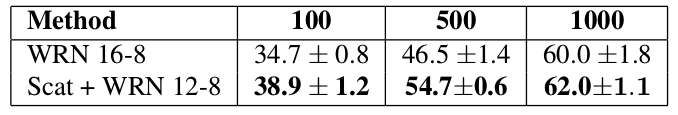
\includegraphics[width=0.6\textwidth]{images/results_scaling_the_scattering.png}
		\end{figure}
	\end{frame}
	%
	\section{Models/Experiments}
	\subsection{ } % for the dots - there most probably is a more elegant solution.
	\begin{frame}{Single Shot MultiBox Detector (SSD)}
		\begin{figure}
			\centering
			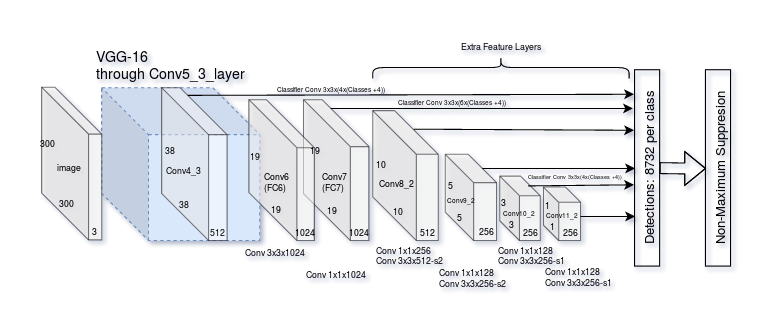
\includegraphics[width=\textwidth]{images/simple_ssd.png}
		\end{figure}
	\end{frame}
	%
	\begin{frame}{Sequential Scattering SSD}
		\begin{block}{}
			\begin{itemize}
				\item Scattering is applied before data is piped through SSD
			\end{itemize}
		\end{block}
		\begin{figure}
			\centering
			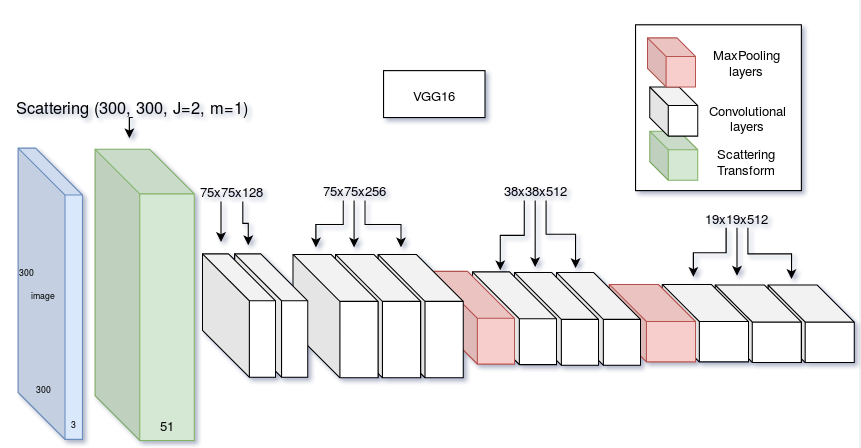
\includegraphics[width=0.9\textwidth]{images/sequential_scattering_ssd.png}
		\end{figure}
	\end{frame}
	%
	\begin{frame}{Parallel Scattering SSD}
		\begin{block}{}
			\begin{itemize}
				\item Data is piped through scattering and standard SSD and continuously merged at different stages
			\end{itemize}
		\end{block}
		\begin{figure}
			\centering
			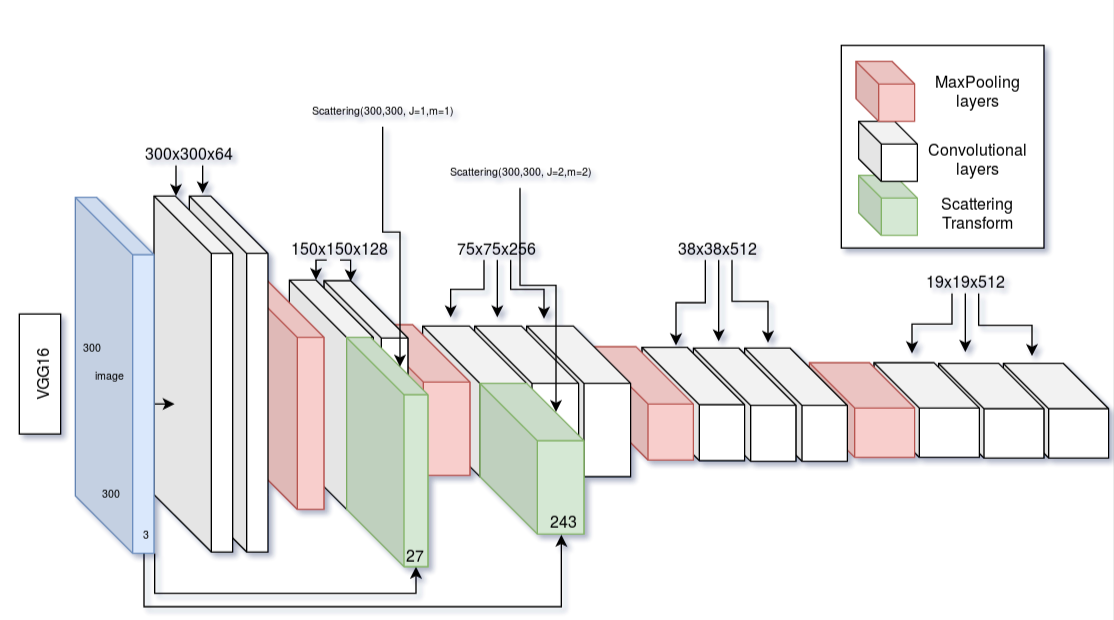
\includegraphics[width=0.8\textwidth]{images/parallel_scattering_vgg.png}
		\end{figure}
	\end{frame}
	%
	\begin{frame}{Datasets - VOC}
		\begin{figure}[!htb]
			\centering
			\begin{tabular}{ccc}
				\subfloat[]{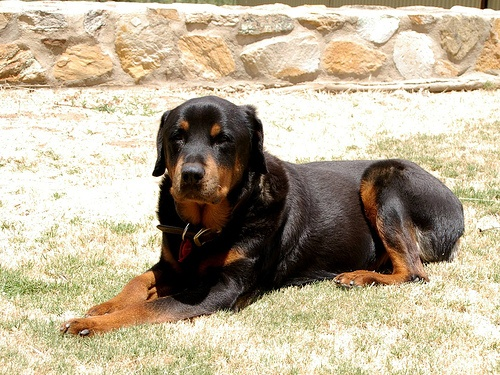
\includegraphics[width=3cm]{images/VOC_sample_1.jpg}} 
				& \subfloat[]{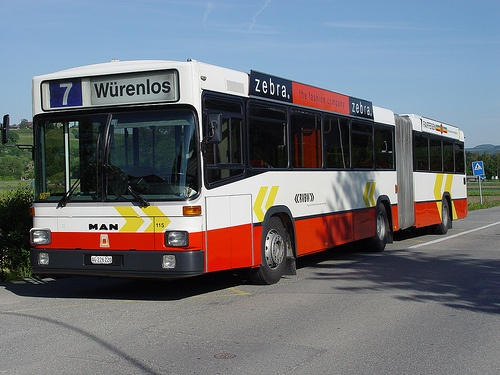
\includegraphics[width=3cm]{images/VOC_sample_2.jpg}}&
				\subfloat[]{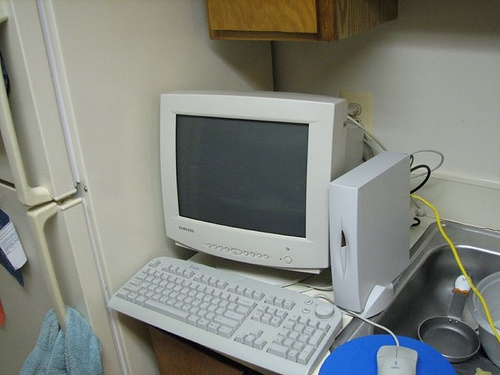
\includegraphics[width=3cm]{images/VOC_sample_3.jpg}}
			\end{tabular}
			\caption{Three samples from the PASCAL VOC dataset showing a dog, bus and TV monitor from left to right.}
			\label{fig:VOC_samples}
		\end{figure}
	\end{frame}
	%
	\begin{frame}{Datasets - Kitti}
		\begin{figure}[!htb]
			\centering
			\begin{tabular}{cc}
				\subfloat[]{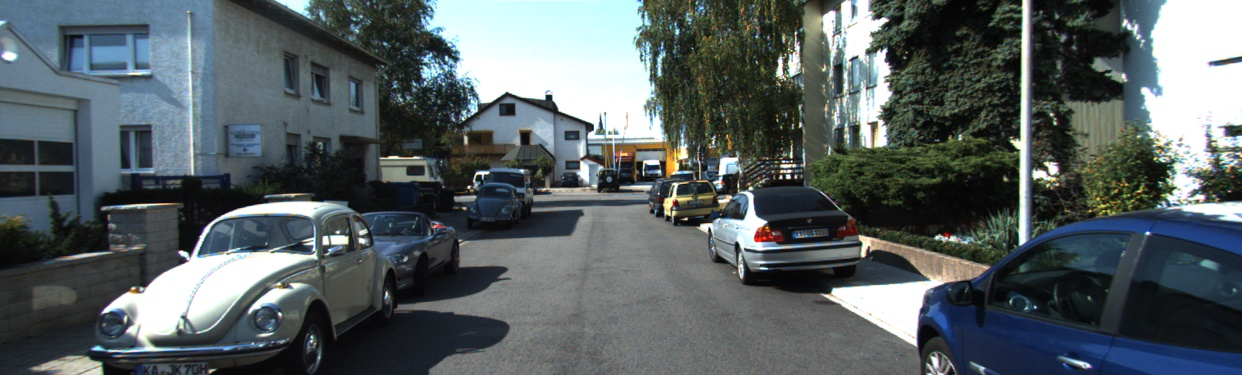
\includegraphics[width=4cm]{images/kitti_sample_1.jpg}} 
				& \subfloat[]{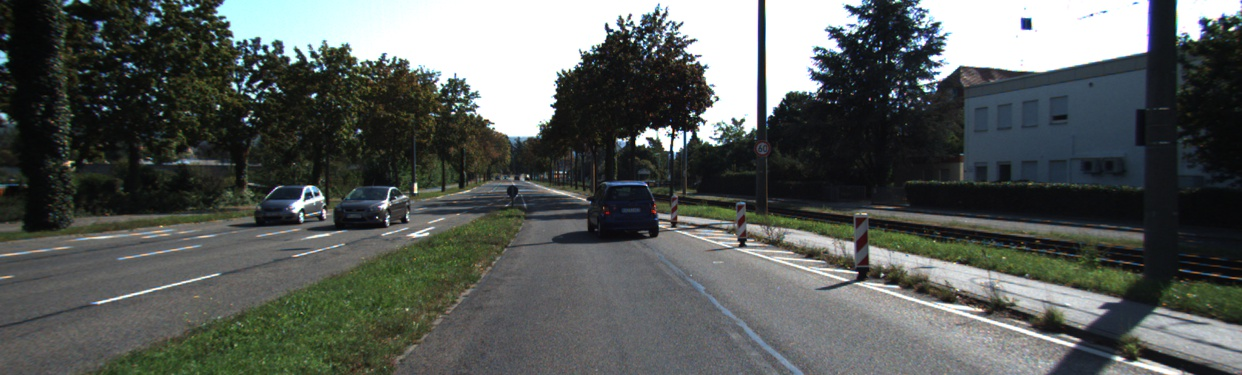
\includegraphics[width=4cm]{images/kitti_sample_2.jpg}} \\
				\subfloat[]{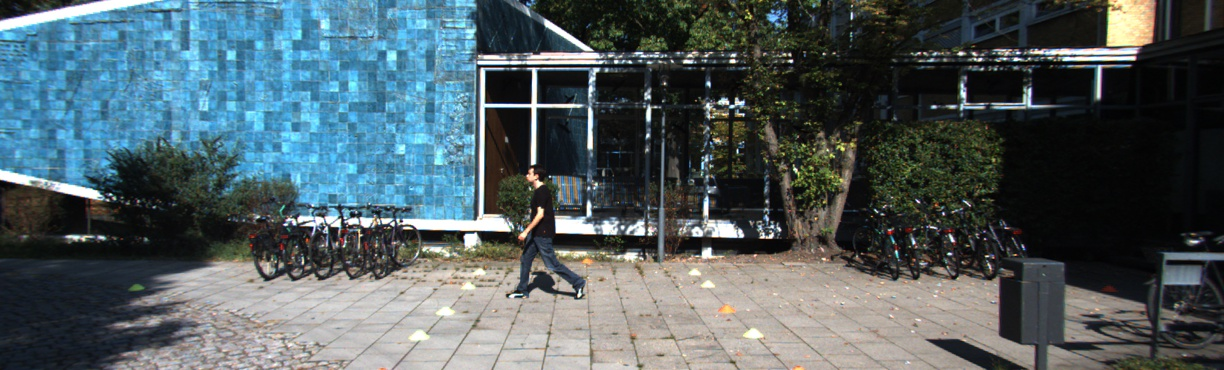
\includegraphics[width=4cm]{images/kitti_sample_3.jpg}} 
				& \subfloat[]{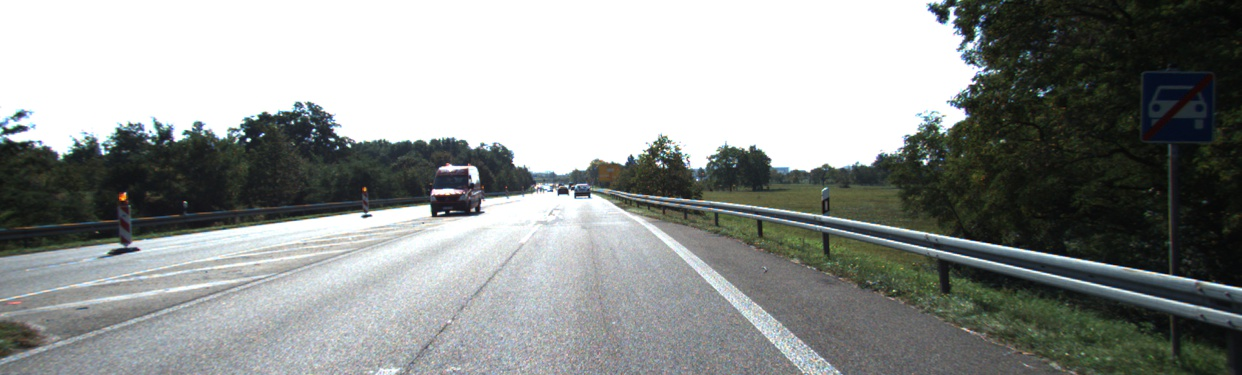
\includegraphics[width=4cm]{images/kitti_sample_4.jpg}} 
			\end{tabular}
			\caption{Four samples from the KITTI dataset.}
			\label{fig:kitti_samples}	
		\end{figure}
	\end{frame}
	%
	\begin{frame}{Datasets - Toydata}
		\begin{figure}[!htb]
			\centering
			\begin{tabular}{cccc}
				\subfloat[]{\fbox{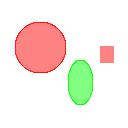
\includegraphics[width=2.2cm]{images/toy_data/0010001.jpg}}} 
				& \subfloat[]{\fbox{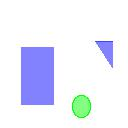
\includegraphics[width=2.2cm]{images/toy_data/0010002.jpg}}} &
				\subfloat[]{\fbox{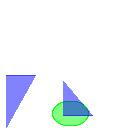
\includegraphics[width=2.2cm]{images/toy_data/0010005.jpg}}}  &
				\subfloat[]{\fbox{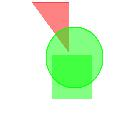
\includegraphics[width=2.2cm]{images/toy_data/0010006.jpg}}} 
			\end{tabular}
			\caption{Four samples from the toy data set.}
			\label{fig:toy_data_samples}
		\end{figure}
	\end{frame}
	%
	\begin{frame}{toy datasets}
		\begin{block}{Idea}
			Test if the promised equivariances/invariances hold on specifically created toy datasets
		\end{block}
		\begin{itemize}
			\item Translation dataset
			\item Scale dataset
			\item Rotation dataset
			\item Deformation dataset
		\end{itemize}
	\end{frame}
	%
	\begin{frame}{Translation dataset}
		\begin{figure}[!htb]
			\centering
			\begin{tabular}{cccc}
				\subfloat[]{\fbox{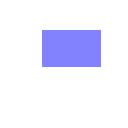
\includegraphics[width=2.2cm]{images/translation_data/0000017_00.jpg}}} 
				& \subfloat[]{\fbox{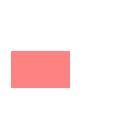
\includegraphics[width=2.2cm]{images/translation_data/0000017_03.jpg}}} &
				\subfloat[]{\fbox{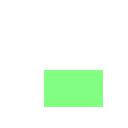
\includegraphics[width=2.2cm]{images/translation_data/0000017_09.jpg}}}  &
				\subfloat[]{\fbox{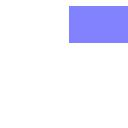
\includegraphics[width=2.2cm]{images/translation_data/0000017_10.jpg}}} 
			\end{tabular}
			\caption{Four samples from the translation toy data set. a) is the base image; b) -d) are the translated versions}
			\label{fig:translation_samples}
		\end{figure}
	\end{frame}
	%
	\begin{frame}{Scale dataset}
		\begin{figure}[!htb]
			\centering
			\begin{tabular}{cccc}
				\subfloat[]{\fbox{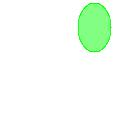
\includegraphics[width=2.2cm]{images/scale_data/0000000_00.jpg}}} 
				& \subfloat[]{\fbox{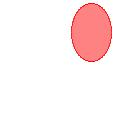
\includegraphics[width=2.2cm]{images/scale_data/0000000_03.jpg}}} &
				\subfloat[]{\fbox{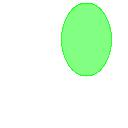
\includegraphics[width=2.2cm]{images/scale_data/0000000_09.jpg}}}  &
				\subfloat[]{\fbox{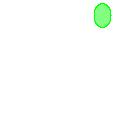
\includegraphics[width=2.2cm]{images/scale_data/0000000_10.jpg}}} 
			\end{tabular}
			\caption{Four samples from the scale toy data set. a) is the base image; b) -d) are the scaled versions}
			\label{fig:scale_samples}
		\end{figure}
	\end{frame}
	%
	\begin{frame}{Rotation dataset}
		\begin{figure}[!htb]
			\centering
			\begin{tabular}{cccc}
				\subfloat[]{\fbox{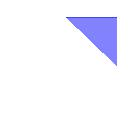
\includegraphics[width=2.2cm]{images/rotation_data/0000000_00.jpg}}} 
				& \subfloat[]{\fbox{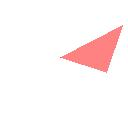
\includegraphics[width=2.2cm]{images/rotation_data/0000000_03.jpg}}} &
				\subfloat[]{\fbox{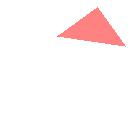
\includegraphics[width=2.2cm]{images/rotation_data/0000000_09.jpg}}}  &
				\subfloat[]{\fbox{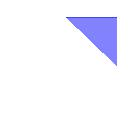
\includegraphics[width=2.2cm]{images/rotation_data/0000000_10.jpg}}} 
			\end{tabular}
			\caption{Four samples from the rotation toy data set. a) is the base image; b) -d) are the rotated versions}
			\label{fig:rotation_samples}
		\end{figure}
	\end{frame}	
	%
	\begin{frame}{Deformation dataset}
		\begin{figure}[!htb]
			\centering
			\begin{tabular}{cccc}
				\subfloat[]{\fbox{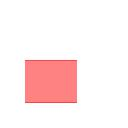
\includegraphics[width=2.2cm]{images/deformation_data/0000001_00.jpg}}} 
				& \subfloat[]{\fbox{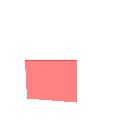
\includegraphics[width=2.2cm]{images/deformation_data/0000001_03.jpg}}} &
				\subfloat[]{\fbox{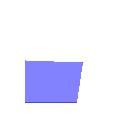
\includegraphics[width=2.2cm]{images/deformation_data/0000001_09.jpg}}}  &
				\subfloat[]{\fbox{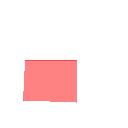
\includegraphics[width=2.2cm]{images/deformation_data/0000001_10.jpg}}} 
			\end{tabular}
			\caption{Four samples from the deformation toy data set. a) is the base image; b) -d) are the deformed versions}
			\label{fig:deformation_samples}
		\end{figure}
	\end{frame}
	%
	\begin{frame}{Experiments}
		\begin{enumerate}
			\item Performance on all datasets
			\item Performance on very small datasets with low training time
			\item Time consumption per forward pass
		\end{enumerate}
	\end{frame}
	%
	\begin{frame}{Results - Comparison}
		\begin{figure}[!htb]
			\centering
			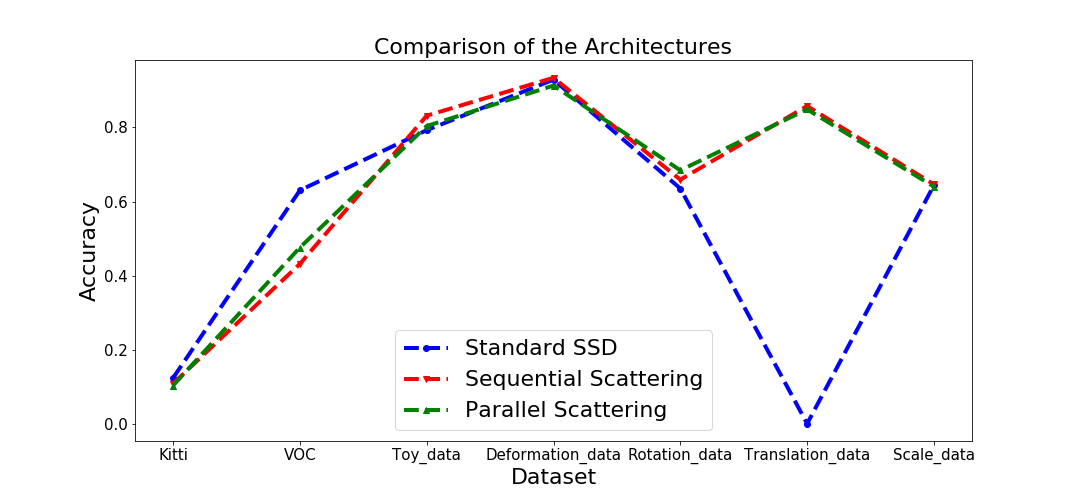
\includegraphics[width=\textwidth]{images/comparison_scaled.png}
			\label{fig:comparison}
			\caption{Final comparison on all datasets}
		\end{figure}
	\end{frame}
	%
	\begin{frame}{Results - Small data experiments}
		\begin{table}[!htb]
			\centering
			\resizebox{\columnwidth}{!}{
			\begin{tabular}{lccc}
				\toprule
				Dataset & standard & sequential & parallel \\
				\midrule
				Toy\_data\_small (25k) &   0.630 $\pm$ 0.008 & \textbf{0.759 $\pm$ 0.004}  & 0.411 $\pm$  0.012 \\
				Toy\_data\_small (5k) & 0.043 $\pm$ 0.007 & \textbf{0.121 $\pm$ 0.027} &  0.003 $\pm$  0.001 \\
				\hdashline
				VOC (25k)& \textbf{0.317 $\pm$ 0.011} &  0.053 $\pm$  0.006 &  0.013 $\pm$  0.001 \\
				VOC (5k)&  \textbf{0.025 $\pm$ 0.001} & 0.011 $\pm$ 0.007 &  0.004 $\pm$  0.000 \\
				\bottomrule
			\end{tabular}
			}
			\label{table:small_data_experiments2}
		\end{table}
		
%		\begin{table}[!htb]
%			\centering
%			%\caption{Results of the small data experiments. Mean and standard deviation of the accuracy are denoted for every combination of features that were measured.}
%			\begin{tabular}{lllrr}
%				\toprule
%				Dataset & epochs &           network type &   Mean &  Std\_dev \\
%				\midrule
%				Toy\_data\_small &    25k &               standard &  0.630 &    0.008 \\
%				Toy\_data\_small &    25k &  sequential\_scattering &  0.759 &    0.004 \\
%				Toy\_data\_small &    25k &    parallel\_scattering &  0.411 &    0.012 \\
%				Toy\_data\_small &     5k &               standard &  0.043 &    0.007 \\
%				Toy\_data\_small &     5k &  sequential\_scattering &  0.121 &    0.027 \\
%				Toy\_data\_small &     5k &    parallel\_scattering &  0.003 &    0.001 \\
%				\hdashline
%				VOC &    25k &               standard &  0.317 &    0.011 \\
%				VOC &    25k &  sequential\_scattering &  0.053 &    0.006 \\
%				VOC &    25k &    parallel\_scattering &  0.013 &    0.001 \\
%				VOC &     5k &               standard &  0.025 &    0.001 \\
%				VOC &     5k &  sequential\_scattering &  0.011 &    0.007 \\
%				VOC &     5k &    parallel\_scattering &  0.004 &    0.000 \\
%				\bottomrule
%			\end{tabular}
%			\label{table:small_data_experiments}
%		\end{table}
	\end{frame}
	%
	\begin{frame}{Results - Timing experiments}
		\begin{table}[!htb]
			\centering
			%\caption{Mean and standard deviation (std.) of 100 runs of the timing evaluation for the normal SSD, the sequential and the parallel scattering SSD are shown. Means are reported in seconds. The sequential scattering is faster than the standard approach. Both are significantly faster than the parallel scattering.}
			\begin{tabular}{lcc}
				\toprule
				network type & mean & std. \\
				\midrule
				normal SSD & 0.236 & 0.004 \\
				sequential scattering & 0.178 & 0.004 \\
				parallel scattering & 1.499 & 0.002 \\
				\bottomrule
			\end{tabular}
			\label{table:timing_evaluation}
		\end{table}
	\end{frame}
	%
	\section{Outro}
	\subsection{ } % for the dots - there most probably is a more elegant solution.
	\begin{frame}{Conclusion}
		\begin{itemize}
			\item The \textbf{sequential} Scattering Transform is faster and more robust method for some applications
			\item The \textbf{parallel} Scattering Transform is significantly slower and does not provide the supposed benefits 
			\item (In a follow-up experiment the parallel scattering gets the best of both worlds while taking twice as long per forward pass)
		\end{itemize}
	\end{frame}
	\begin{frame}{Questions}
		\begin{center}
			\huge{Questions?}
		\end{center}
	\end{frame}
	%
	\begin{frame}[shrink=30]{References}
		\cite{scatteringTransform2012}, \cite{InvariantScatteringTextureDiscrimination2013}, \cite{DeepRotoTranslation2014}, 
		\cite{ScalingTheScatteringTransform2017},
		\cite{3DScatteringTransformNeuro2017}
		\bibliographystyle{alpha}
		\small\bibliography{bibliography}
	\end{frame}
	%
	\section{Appendix}
	%the results of the new parallel scattering and a visualization
	
	%
	%Some further equations
	\begin{frame}{Backup Equations - number of filters}
		\begin{equation}
		i \cdot (1 + JL) 
		\label{eq:order1_num_filters}
		\end{equation} 
		\begin{equation}
		i \cdot (1 + JL + \frac{1}{2}J(J-1)L^2)
		\label{eq:order2_num_filters}
		\end{equation}
		\begin{itemize}
			\item Let $J=2, L=8, N,M=32,32$ for a RGB image.
			\item number of outputs of the scattering network for $m=1$:
			$$ 3\cdot (1 + 2 * 8) = 51$$
			\item number of outputs of the scattering network for $m=2$:
			$$ 3 \cdot (1 + 16 + 0.5*2*1 * 64) = 243$$
			\item all outputs of size 8x8
		\end{itemize}
	\end{frame}
	%
	%more equations?
	\begin{frame}{More definitions:}
		\begin{itemize}
			\item Central Frequency: \begin{equation*}
			\int_{-\infty}^{\infty} \omega | \Psi(\omega)|^2 d\omega
			\end{equation*}
			where $\Psi$ is the Fourier Transform of the wavelet $\psi$. This is the centre of mass of $|\Psi(\omega)|^2$.
		\end{itemize}
	\end{frame}
	%scattering coefficients for the other datasets
	\begin{frame}{Coefficients - Example 1}
		\begin{figure}[!htb]
			\centering
			\begin{tabular}{cc}
				\subfloat[]{\fbox{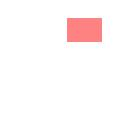
\includegraphics[width=3cm]{images/0000011_00.jpg}}} 
				& \subfloat[]{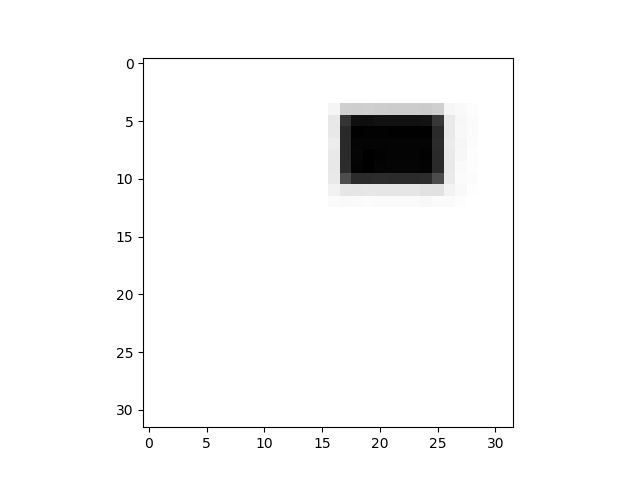
\includegraphics[width=3cm]{images/example1_0ord.png}}\\
				
				\subfloat[]{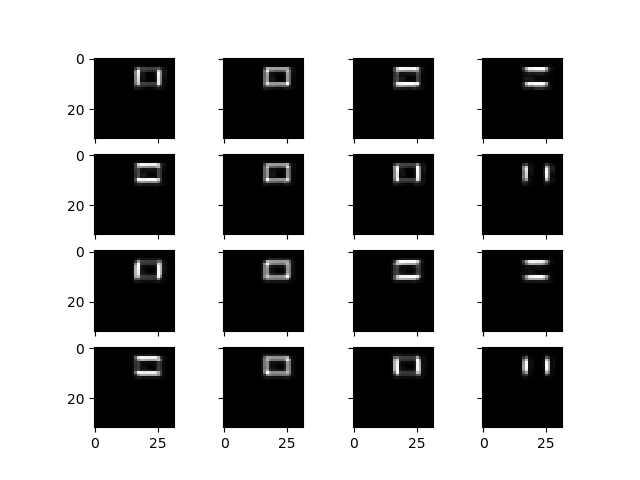
\includegraphics[width=3cm]{images/example1_1ord.png}} &
				\subfloat[]{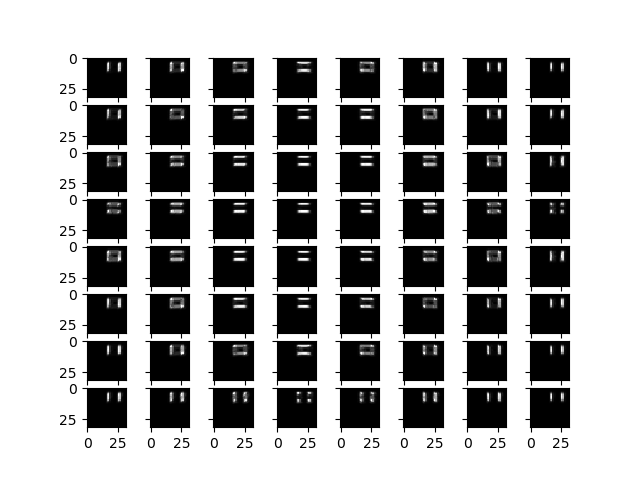
\includegraphics[width=3.5cm]{images/example1_2ord.png}}
			\end{tabular}
			%\caption{Image taken from a toy dataset created for this work. a) Original image; b) 0th order scattering coefficients, i.e. a Gaussian low-pass filter; c) First order scattering coefficients; d) Second order scattering coefficients}
			\label{fig:example1_coefficients}
		\end{figure}
	\end{frame}
	%
	%translated example1 = example2
	\begin{frame}{Coefficients - Example 1 (translated)}
		\begin{figure}
			\centering
			\begin{tabular}{cc}
				\subfloat[]{\fbox{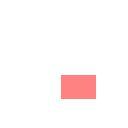
\includegraphics[width=3cm]{images/0000011_03.jpg}}} 
				& \subfloat[]{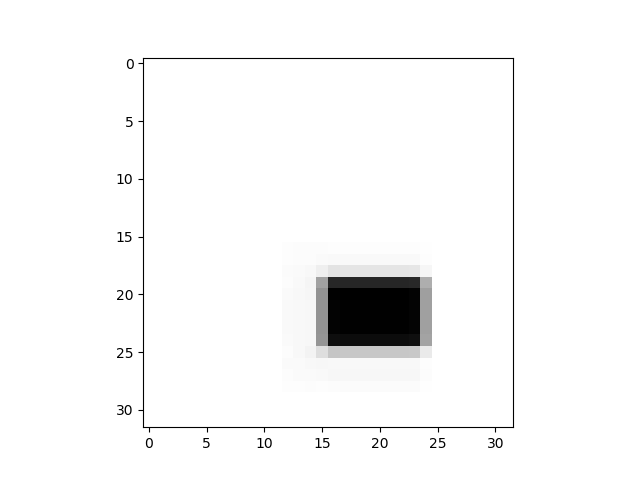
\includegraphics[width=3cm]{images/example2_0ord.png}}\\
				
				\subfloat[]{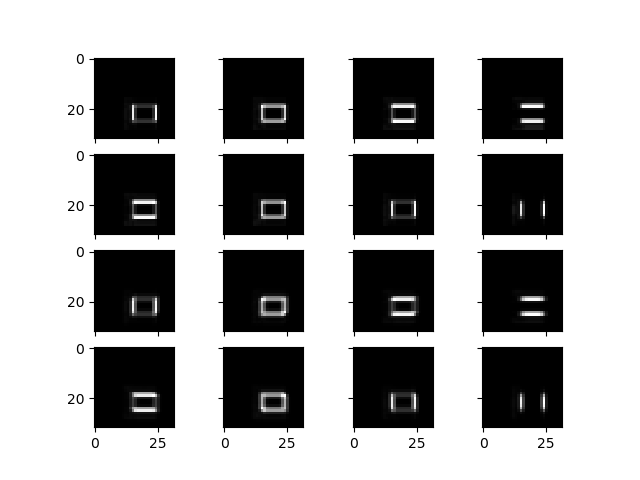
\includegraphics[width=3cm]{images/example2_1ord.png}} &
				\subfloat[]{\includegraphics[width=3.5cm]{images/example2_2ord.png}}
			\end{tabular}
			%\caption{Image taken from a toy dataset created for this work. a) Original image; b) 0th order scattering coefficients, i.e. a Gaussian low-pass filter; c) First order scattering coefficients; d) Second order scattering coefficients}
			\label{fig:example2_coefficients}
		\end{figure}
	\end{frame}
	
	%first ellipse
	\begin{frame}{Coefficients - Ellipse}
		\begin{figure}
			\centering
			\begin{tabular}{cc}
				\subfloat[]{\fbox{\includegraphics[width=3cm]{images/0000027_09.jpg}}} 
				& \subfloat[]{\includegraphics[width=3cm]{images/example1e_0ord.png}}\\
				
				\subfloat[]{\includegraphics[width=3cm]{images/example1e_1ord.png}} &
				\subfloat[]{\includegraphics[width=3.5cm]{images/example1e_2ord.png}}
			\end{tabular}
			%\caption{Image taken from a toy dataset created for this work. a) Original image; b) 0th order scattering coefficients, i.e. a Gaussian low-pass filter; c) First order scattering coefficients; d) Second order scattering coefficients}
			\label{fig:example1e_coefficients}
		\end{figure}
	\end{frame}
	
	%second ellipse
	\begin{frame}{Coefficients - Ellipse (scaled)}
		\begin{figure}
			\centering
			\begin{tabular}{cc}
				\subfloat[]{\fbox{\includegraphics[width=3cm]{images/0000027_10.jpg}}} 
				& \subfloat[]{\includegraphics[width=3cm]{images/example2e_0ord.png}}\\
				
				\subfloat[]{\includegraphics[width=3cm]{images/example2e_1ord.png}} &
				\subfloat[]{\includegraphics[width=3.5cm]{images/example2e_2ord.png}}
			\end{tabular}
			%\caption{Image taken from a toy dataset created for this work. a) Original image; b) 0th order scattering coefficients, i.e. a Gaussian low-pass filter; c) First order scattering coefficients; d) Second order scattering coefficients}
			\label{fig:example2e_coefficients}
		\end{figure}
	\end{frame}
	


\end{document}
